\def\DevnagVersion{2.15}% Created by: Pranjal Singh
\documentclass{article}
\usepackage[margin=1.2in]{geometry}
\usepackage{parskip}
\usepackage{graphicx}
\usepackage{epsfig}
\usepackage{amsmath}
\usepackage{hyperref}
\usepackage{polyglossia}
\usepackage{devanagari}
\setdefaultlanguage{english} 
\setotherlanguage{sanskrit} 
\usepackage{xltxtra}
\pagestyle{plain}

\newfontinstance
\sahadeva [Script=Devanagari,Mapping=velthuis-sanskrit]{Sahadeva}
\newcommand{\mangaluni}[1]{{\mangal\textsanskrit{#1}}}


\title{\huge{An Empirical Study of Cross-Lingual Unsupervised Alignment Based on Syntactic Features}}
\author{Pranjal Singh \\ \\  Advisor: Prof. Amitabha Mukerjee \\ Dept. of Computer Science \& Engg.\\ IIT Kanpur, India \\ \{spranjal,amit\}@iitk.ac.in}
\date{\today}
\begin{document}
\maketitle
\begin{abstract}
In this work, we experiment with three approaches to extract relationship between cross-lingual clusters and sentences. While other work have mainly focused on few features such as predicates and have not directly looked into the whole document, we consider the whole document and not merely look at few features. Moreover, our work is more on a focused data,i.e. data concentrated on very few topics. We have used unsupervised learning of Natural Languages and concentrated on Hindi and English, though it can be extended to any language.
\end{abstract}\setlength{\parindent}{0.25in}

\section{Introduction}
We are facing an ever increasing volume of text documents. The abundant texts flowing over the Internet, huge collections of documents in digital libraries and repositories, and digitized personal information such as blog articles and emails are piling up quickly everyday. The ability to align text from different languages is an important problem of Natural Language Processing(NLP). With increasing number of textual contents in the universe, it has become quite important to identify similar contents in two languages.\\
We have used unsupervised methods of learning due to their advantage over supervised methods. They do not require an annotated corpus which proves to be quite costly. Also the corpus used has been manually built by us which includes a Hindi corpus and an English corpus containing articles on \emph{Coal Scam}. Hindi corpus contains around 30000 lines whereas English corpus consists of over 50000 lines. Here each line is treated as a document.\\
We have used PLSA to create clusters from our focused corpora of both the languages to analyze whether there is word level alignment among both the languages. For that we have used words as our features and have created term-frequency(\emph{tf}) matrix. For creation of feature vectors, we have done some preprocessing of corpus and removed stopwords and symbols. We have ignored stemming in this work because we do not want to interfere with the syntax of the language.\newpage
We have also used ADIOS in our work to derive some syntactic features hidden in both the corpora. This analysis can give intrinsic details about any type of alignment hidden in both the corporas which we expect to be present because they are focused corporas.\\
We know that a child learns about a topic from only few words which are most influencing in describing an event. These are mainly the most frequent words or bigrams. These most frequent words are not the stop words but Nouns, Adjectives or Verbs. \\
This work can thus prove to be quite useful in simplification of a large corpus for understanding of a child who doesn't know one language but knows the other one. The alignment present in the clusters could prove to be an integral part in this learning. We extract important words from a corpus describing it. This can also roughly summarize what a document is talking about.\\
Note that the word ‘feature’ in ‘distributional features’ indicates the value assigned to a word, which is somewhat different from its usual meaning, i.e. the element used to characterize a document.
The next section talks about similar work in this field. Then we have discussed about PLSA, followed by ADIOS Algorithm, Implementation Details, Results and Future Work.

\section{Relevant Work}
The previous relevant work in this field have been mainly on few features rather than whole document and looking all features. no work has been done using PLSA or ADIOS on "concentrated corpus" and especially with Hindi. The previous works have mainly looked at sentence level alignment which doesn't prove to be very helpful in understanding a large document by a child. \\
Our main contribution is a general technique for inducing cross lingual distributed representations.\\
Ji et.al. have looked at bilingual predicate cluster acquisition. They have proposed an inductive learning framework to automatically augment background data for low-confidence events and then conduct global inference. This inductive learning approach matches the procedure of human knowledge acquisition and foreign language education: analyze information from specific examples and then discover a pattern or draw a conclusion; attempt synonyms to convey/learn the meaning of an intricate word.\\
Tackstrom et.al. have looked at Cross-lingual Word Clusters for Direct Transfer of Linguistic Structure. They provide an algorithm for inducing cross-lingual clusters and have shown that features derived from these clusters significantly improve the accuracy of cross-lingual structure prediction.\\

\section{PLSA:Probabilistic Latent Semantic Analysis}
\normalsize Probabilistic Latent Semantic Analysis(pLSA) is a technique from the category of topic models. Its main goal is to model co occurrence information under a probabilistic framework in order to discover the underlying semantic structure of the data.\\
For this particular application, our training data is a corpus|a large set of documents|that is usually represented in the
form of a document-term matrix (this indicates the number of times each word appears in each document). The goal of pLSA is to use this
co-occurrence matrix to extract the so-called "topics" and explain the documents as a mixture of them.
PLSA considers that our data can be expressed in terms of 3 sets of variables:\\
\begin{itemize}
\item Document{s}: d \ensuremath{{\varepsilon} D = \{d_{1},. . . .,d_{N}\}} observed variables. Let N be their number, defined by the size of our given corpus.
\item Words: w \ensuremath{{\varepsilon} W = \{w_{1},. . . .,w_{M}\}} observed variables. Let M be the number of distinct words from the corpus.
\item Topics: z \ensuremath{{\varepsilon} Z = \{z_{1},. . . .,z_{K}\}} latent(or hidden) variables. Their number, K, has to be specified a priori.
\end{itemize}

A generative process for the documents is:
\begin{itemize}
\item First we select a document \ensuremath {d_{n}} with probability \ensuremath{P(d)}.
\item For each word \ensuremath {w_{i}, i {\varepsilon} \{1,. . . .,N_{w}\}} in the document \ensuremath{d_{n}}:
\begin{itemize}
\item Select a topic \ensuremath{z_{i}} from a multinomial conditioned on the given document with probability \ensuremath {P(z|d_{n})}.
\item Select a word \ensuremath{w_{i}} from a multinomial conditioned on the previous chosen topic with probability \ensuremath {P(w|z_{i})}.
\end{itemize}
\end{itemize}

There are some important assumptions made by the presented model:
A generative process for the documents is:

\begin{itemize}
\item Bag-of-words. Intuitively, each documents regarded as an unordered collection of words. More precisely, this means that the joint variable (d,w) is independently sampled and, consequently, the joint distribution of the observed data will factorize
as a product:\\ 
\begin{center} P(D,W) = \ensuremath{\prod_{(d,w)} P(d,w)} \end{center}
\item Conditional independence. This means that words and documents are conditionally independent given the topic:
\ensuremath {P(w|d,z)} = \ensuremath {P(w|z)P(d|z)} or \ensuremath {P(w|d,z)} = \ensuremath{P(w|z)}. (This can be easily proved by using d-separation into our graphical model: the path from d to w is blocked by z.)
\end{itemize}
%Using the conditional independence assumption, we obtain:\\
%\ensuremath{P(w|d)} = \ensuremath{\sum_{z \ensuremath{\varepsilon} Z}} \ensuremath{P(w|z)P(z|d)}\\
%\ensuremath{P(w,d)} = \ensuremath{\sum_{z \ensuremath{\varepsilon} Z}} \ensuremath{P(z)P(d|z)P(w|z)}
%\newline \\
The predictive probability of pLSA mixture model is denoted by \ensuremath{P(w|d)}, so the objective function is given by the following expression:\\ L = \ensuremath{\prod_{(d,w)} P(w|d)} = \ensuremath{\prod_{(d \ensuremath{\varepsilon} D)}\prod_{(w \ensuremath{\varepsilon} W)} P(w|d)^{n(d,w)}}\newline \\

where \ensuremath{n(d|w)} represents the observed frequencies, the number of times word w appears in document d. This is a non-convex optimization problem and it can be solved by using Expectation-Maximization (EM) algorithm for the log-likelihood:\\

\begin{center}
\textbf{M = \ensuremath{\log L} = \ensuremath{\prod_{(d \ensuremath{\varepsilon} D)}\prod_{(w \ensuremath{\varepsilon} W)} n(d,w) . \ensuremath{\log \ensuremath{\sum_{z \ensuremath{\varepsilon} Z}} P(w|z)P(z|d) }}}
\end{center}

\section{ADIOS Algorithm}
The algorithm which is used in this project is ADIOS(Automatic Distillation Of Structure).
The following is a small description of the MEX criterion which is used as a distillation tool for extracting the most significant patterns in the data .\\ \\
{\large \bf The MEX Criterion}
\\
In this criterion we create a pseudo graph(a non-simple graph in which both loops and multiple edges are permitted) where the sentences correspond to the different paths and vertices are the unique lexicon entries, augmented by two special symbols 'begin' and 'end'. The following diagram indicates structure that we seek, namely, the bundling of paths, signifying a relatively high probability associated with a sub-structure that can be identified as a pattern.\\
\begin{center}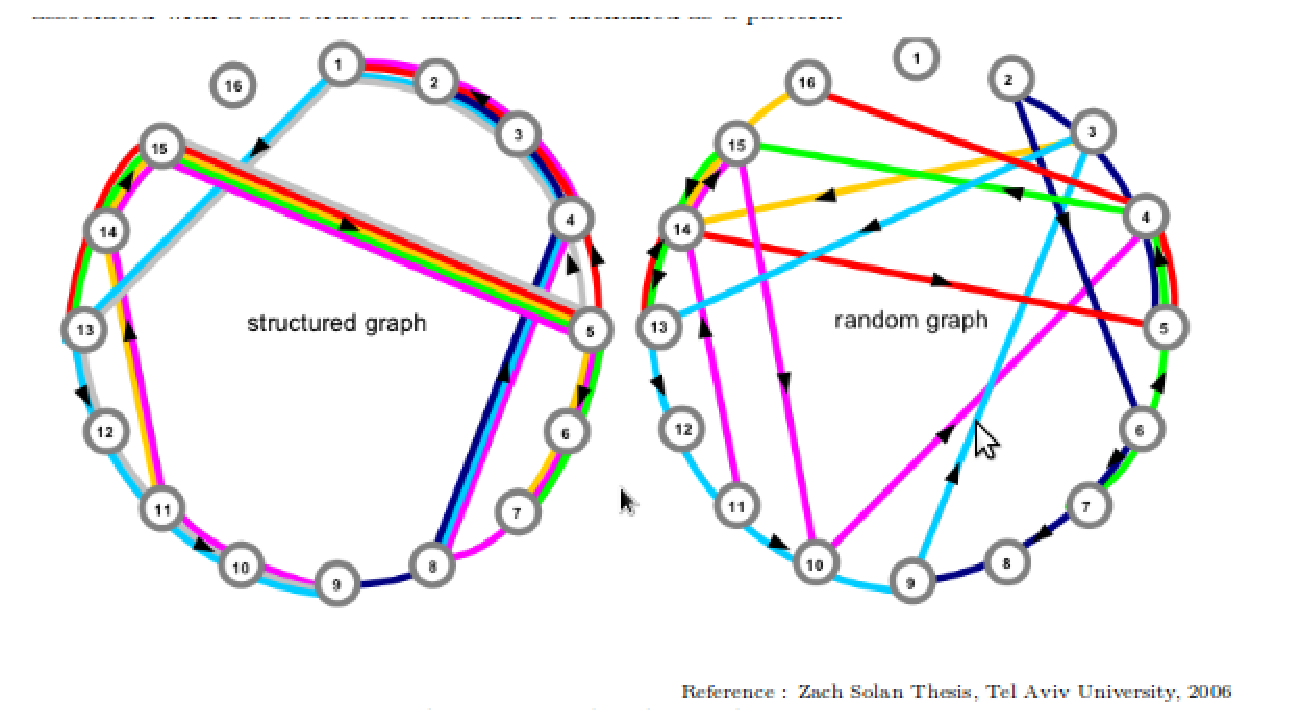
\includegraphics[width=10cm]{graph.eps}\end{center}
	   
\hfill {\scriptsize Reference : Zach Solan Thesis, Tel Aviv University, 2006}
\\
Firstly we define a search path $S(e1 -> e2 -> ... -> ek ) = (e1 ; ek )$
\\Next we define two probability functions $P_R$(right) and $P_L$(left) as:
\\
$P_R (e_i;e_j ) = p(e_j |e_i e_{i+1} e_{i+2} ...e_{j−1} ) = l(e_{i} ; e_{j} ) / l(e_{i} ; e_{j−1} )$
\\
where $l(e_i ; e_j )$ is the number of occurrences of sub-paths $(e_i ; e_j )$ in the graph .
\\
\\Similarly proceeding from left we have
\\
$P_L (e_j ; e_i ) = p(e_i |e_{i+1} e_{i+2} ...e_{j−1} e_j ) = l(e_j ; e_i )/ l(e_j ; e_{i+1} )$
\\ \\
We define decrease ratio, $D_R (e_i ; e_j )$, whose value at $e_j$ is $D_R (e_i ; e_j ) = P_R (e_i ; e_j )/P_R (e_i ; e_{j−1} )$
and another decrease ratio, $D_L (e_j ; e_i ) = P_L (e_j ; e_i )/P_L (e_{j+1} ; e_i )$
\\
The algorithm calculates $P_L$ and $P_R$ from all possible starting points and this defines a matrix of the form:
\\
\begin{equation}
  M_{ij}(S)=\begin{cases}
    P_R(e_i;e_j), & \text{if $i>j$}.\\
    P_L(e_j;e_i), & \text{if $i<j$}.\\
    P(e_i), & \text{if $i=j$}.
  \end{cases}
\end{equation}
\begin{center}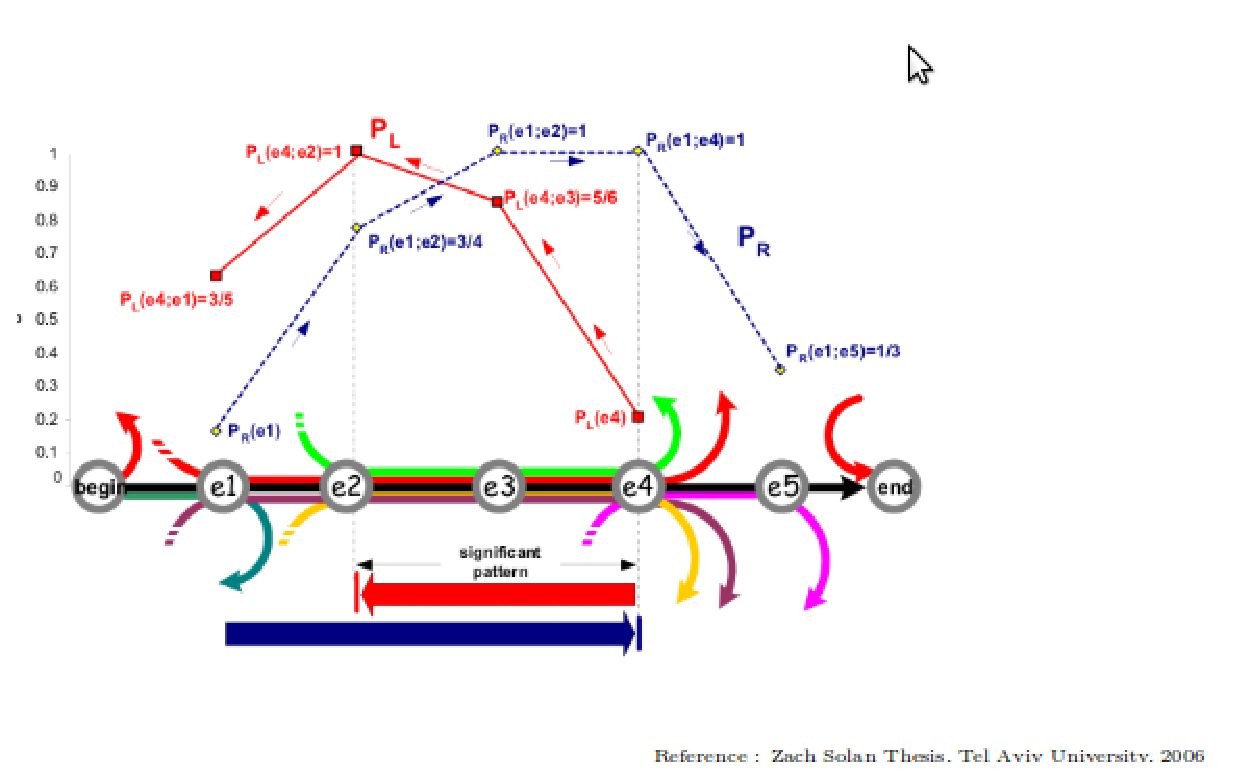
\includegraphics[width=12cm]{pattern.eps}\end{center}

\hfill {\scriptsize Reference : Zach Solan Thesis, Tel Aviv University, 2006}\\
\begin{center}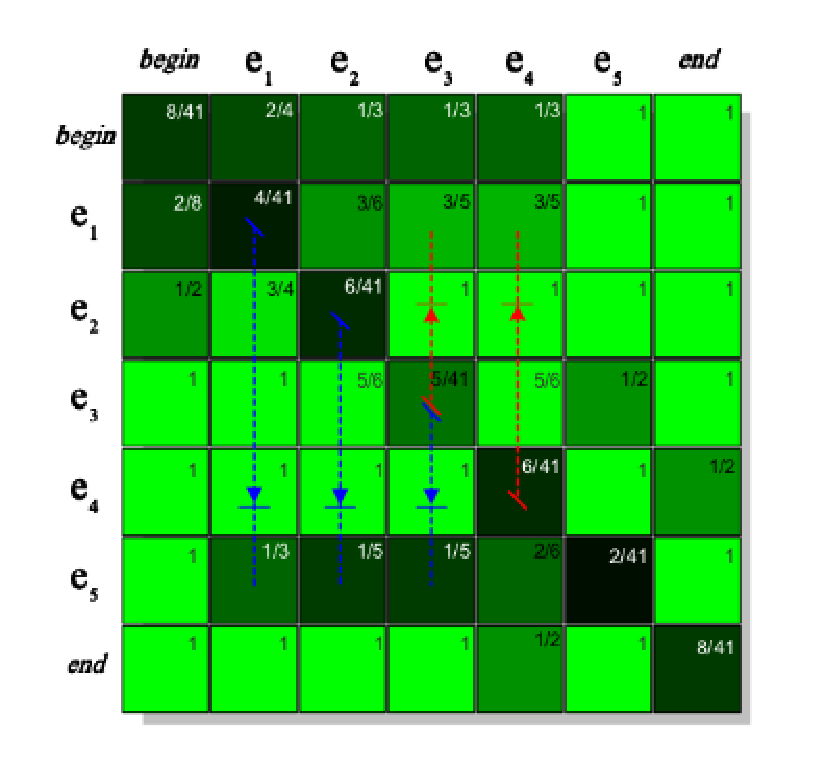
\includegraphics[width=7cm,height=7cm]{a.eps}\end{center}

\hfill {\scriptsize Reference : Zach Solan Thesis, Tel Aviv University, 2006}\\

The algorithm then identifies the leading pattern from the matrix by examining the $D_R$ and $D_L$ and is returned as the outcome of search in question.

\textbf{The ADIOS Algorithm}
\\The algorithm works in three steps:
\begin{enumerate}
 \item INITIALIZATION: sentence loading
 \item PATTERN DISTILLATION: iterative search for significant patterns which are added to lexicons as new units
 \item GENERALIZATION: it generates more and more candidate pattern to be considered by pattern distillation
\end{enumerate} 
So an overview of ADIOS Algorithm is as follows:
\begin{enumerate}
\item {\bf Initialization} (load all sentences)
\item repeat
\item
\begin{tabbing}
 	for \= all m = 1 : N do {N is the number of paths in the graph}\\
	\> {\bf Pattern Distillation(m)} (Identifies new significant 	patterns in search-path m using the MEX criterion) 	\\
	\>	{\bf Generalization(m)} (Generate new pattern candidates for search-path (m))\\
	end for
\end{tabbing}
\item until no further significant patterns are found
\end{enumerate}

\section{Distributional Features}
Distributional Features are motivated by the so-called Distributional Hypothesis:\\ \\
\emph{“The degree of semantic similarity between two linguistic expressions A and B is a function of the similarity of the linguistic contexts in which A and B can appear”.}\footnote{[ Z. Harris (1954) Distributional Structure]}
Currently, distributional semantics is especially popular in computational linguistics. However, its origins are grounded in the linguistic tradition. The underlying assumption is that word meaning depends, at least in part, on the contexts in which words are used. Harris proposed the method of distributional analysis as a scientific methodology for linguistics: introduced for phonology, then methodology for all linguistic levels.\\
Structuralists don’t consider meaning an \emph{explanans} in linguistics: too subjective and vague a notion to be methodologically sound. Linguistic units need to be determined by formal means: by their distributional structure. Harris goes one step farther and claims that distributions should be taken as an explanans for meaning itself. Only this can turn semantics into a proper part of the
linguistic science.\\
A distributional semantic model (DSM) is a co-occurrence matrix M where rows correspond to target terms and columns correspond
to context or situations where the target terms appear.\\ \\
\begin{tabular}{| l | l | l | l | l |}
\hline
\textbf{} & \textbf{see} & \textbf{use} & \textbf{hear} & \textbf{.....} \\ \hline
boat & 39 & 23 & 4 & .... \\ \hline
cat & 58 & 4 & 4 & .... \\ \hline
dog & 83 & 10 & 42 & .... \\ \hline
\end{tabular}
\begin{itemize}
\item Distributional vector of ‘dog’: $x_dog$=(83,10,42,...)
\item Each value in the vector is a \emph{feature} or \emph{dimension}
\item The values in a matrix are derived from event frequencies
\end{itemize}

\section{Implementation Details}
The first part consisted of preprocessing of the data used, for this we had to write a script to extract the Sentences from the corpus. 
\subsection{Running ADIOS}
Then as we had most of the code for the ADIOS algorithm, we basically had to understand and use it. For this we really had to have an
understanding of the algorithm as the code had certain parameters which were initially not very clear. Then as the code had lots of
commands, we needed to decide on what to do first (in this the documentation \url{http://adios.tau.ac.il/algorithm.html#Step_By_Step}
was of great help).\\
The first step was to create a Graph which the ADIOS algorithm can train on.\\
The command consisted of following script:\\

{\bf  ./create\_graph.exe -f name.corpus.txt -o name} \\

The second step was to test the Algorithm on a given new unseen corpus \\
Example: \\
{\bf ./adios.exe -a train -i name.idx -g name.grp -E 0.8 -S 0.01 -o name} \\

{\bf Arguments:}\\

-a command     -$>$ select between training (train) testing (test) printing results (print) generating sentences (generate)\\
-E [0..1]      -$>$ the ETA parameter  (Default: 0.8) we used 0.8 and 0.9\\
-S [0..1]      -$>$ the patterns p-value  (Default: 0.01)\\
-C [0..1]      -$>$ the minimal coverage required from a formed Equivalence Class  (Default: 0.65)\\
-A [1..]       -$>$ The largest pattern size: All patterns with size larger than A will be treated as equal in the rewiring process.\\ 
-B {1..]       -$>$ The minimum pattern size\\

{\bf Output files:}\\ \\
\textbf{name.trace.log}: summary of the algorithm progress\\
\textbf{name.results.txt}: list of the acquired patterns and properties

\section{Results}
\subsection{PLSA clusters}
The following is a cluster of size 3 obtained by using PLSA on our corpus which give a clear indication of relationship present 
between lexicons in our focused corpora.
\newline
\\
\newcommand{\saha}[1]{{\sahadeva\textsanskrit{#1}}}
\saha{[koyalaa, aavan.tan, kola, जिंदलa, ब्लॉकa, कंपनियों, कंपनी, हिंडाल्को, ब्लाकa]}\newline
['coal', 'cbi', 'the', 'allocation', 'birla', 'fir', 'block', 'hindalco', 'alleged']\newline 
\\
\saha{[koyalaa, घोटाले, सीबीआई, darja, sarakaara, सीबीआइ, ब्लॉकa, maamale, पूर्वa]}\newline
['minister', 'coal', 'prime', 'bjp', 'the', 'scam', 'government', 'party', 'issue']\newline 
\\
\saha{[जांचa,कोर्टa,koyalaa,sarakaara,रिपोर्टa,सीबीआई,सुप्रीमa,praधानaमंत्री,मंत्री,घोटाले]}\newline
['cbi', 'coal', 'the', 'court', 'ministry', 'report', 'probe', 'files', 'agency', 'government']

\subsection{ADIOS output}

\section{Further Work}
\normalsize  To improve the quality of results, the training should be done with a large corpus as clearly visible in Unsupervised Learning that the cluster of words can be made more accurate by using a large corpus. Also a mixed approach of supervised and unsupervised learning can be brought to use.\\
Currently we have looked only at a focused corpus but in future we plan to extend this work so that we can look at documents with multiple topics and then strengthen the alignment in the concerned languages with smaller alignments.\\
We can extend the method to look for n-gram clusters in the documents which would give much better detail on the document context. Infact with ADIOS and these clusters, we can simplify the documents for the understanding of a child.\\
This work can also be used to identify semantic relations between sentences in different languages. 

\section{Acknowledgement}
\normalsize I thank Prof. Amitabha Mukerjee for his valuable support throughout the project, guiding me from time to time and looking into the project when it was needed. I have used open source available "ADIOS", PLSA code from "Mathieu's blog" and textmining modules in python. I acknowledge you for your support.
\nocite{*}
\bibliography{report}{}
\bibliographystyle{plain}
\end{document}

